\section{Proposed Algorithm} \label{sec:algorithm}

In this section, we overview the existing naive approach used for constructing prefix tries of hereditary stratigraphy markers, and describe the proposed shortcut-based approach developed in this work.
Notation describes hereditary stratigraphy markers as a pair of two properties: \textit{rank} $r$, referring to the generation at which a marker was generated, and \textit{differentia} $d$, referring to the randomly-generated value distinguishing a given marker from others generated at that generation.

\subsection{Naive Trie-Building Algorithm} \label{sec:algorithm:naive}

The naive algorithm treats each organism's sequence of stored rank-differentia pairs as a string: each differentia $d$ constitutes a character at the rank $r$-th string position.
Differentia values missing due to having been overwritten are considered as wildcard characters.

For two rank-differentia strings, common ancestry corresponds to a shared prefix of string characters inherited from their most recent common ancestor (MRCA).
Under this framing, phylogenies correspond to a trie --- a tree-like data structure where each node corresponds to a character in a string, and each path from the root to a leaf node reads out a stored string \citep{fredkin1960trie}.

The first step in naive reconstruction is to sort all organisms in ascending order by number of generations elapsed.
Due to each organism using the same algorithm to determine which markers to overwrite, this order guarantees that any data missing from an organism will also have been discarded by all subsequent organisms.

We initialize an empty trie, consisting of a single root node.
Trie building proceeds by processing organisms one at a time in their sorted order.
For each organism, we iterate through rank-differentia pairs in chronological order.
At each rank-differentia pair, we either continue along the existing trie, branch off to create a new path, or --- in a special case --- address missing information (Algorithm~\ref{alg:old}).

\begin{algorithm}[h]
    \caption{the existing algorithm for creating a phylogenetic tree through hereditary stratigraphy, using a naive trie-building approach}
    \label{alg:old}
    \begin{algorithmic}[1]
        \Require a list of organisms $O$ in ascending order by generations elapsed
        \Function{ReconstructTree}{$O$}
            \State $T \gets$ an empty tree
            \For {$o \in O$} 
                \State $\textsc{TreeInsert}(T, o)$
            \EndFor
            \State \Return $T$
        \EndFunction

        \Function{TreeInsert}{$T, o$}
            \State $n \gets$ root of $T$
            \For{each rank-differentia pair $(r, d) \in o$}
                \While{$r >$ the rank of $n$'s children}
                    \State $n \gets$ the child of $n$ most likely contain $o$
                \EndWhile
                \If{$\exists c \in \operatorname{children}(n) \text{ s.t.} \operatorname{differentia(c) = d}$}
                    \State $n \gets c$
                \Else 
                    \State create a new child $c'$ branching off $n$ 
                    \State $\operatorname{differentia}(c') \gets d$
                    \State $n \gets c'$
                \EndIf
            \EndFor
            \State insert information about $o$ as a child of $n$
        \EndFunction
    \end{algorithmic}
\end{algorithm}

Missing information is recognized as follows.
Suppose we have reached trie node $n$ with rank $r_1$ and must next process rank-differentia pair $(r_2,\; d)$ from current organism $o$.
If any node with rank $r' < r_2$ exists among children of current node $n$, we know that $r'$ must have been deleted from organism $o$ as its record skips directly from $r_1$ to $r_2$.

To maximize reconstruction accuracy in the case of missing data, we must assess which --- if any --- of $n$'s children our missing datum at $r'$ would have likely corresponded to.
Essentially, when reaching missing information, we must infer that information, which we do by looking ahead in the tree.
Specifically, we search forward for the path with the longest successive streak of differentia matching to current organism $o$ \citep{moreno2024analysis}.
If there is no matching path, we simply branch off node $n$ rather than continuing to traverse through its children.

Note that this approach suffers the cost of doing significant extra work to handle missing information.
In the worst case, there could be an exponential number of matching paths to check, owing to the possibility of nested branch-outs at successive wildcard sites.
These searches are repeated for each organism, regardless of whether or not a similar search was already done.
Therefore, we present an improved algorithm that consolidates this extra work into a single step that never needs to be repeated.

\subsection{Proposed Shortcut Algorithm} \label{sec:algorithm:shortcut}

\begin{figure*}
\begin{minipage}{0.74\linewidth}
\centering
\begin{minipage}{0.32\linewidth}
  \centering
  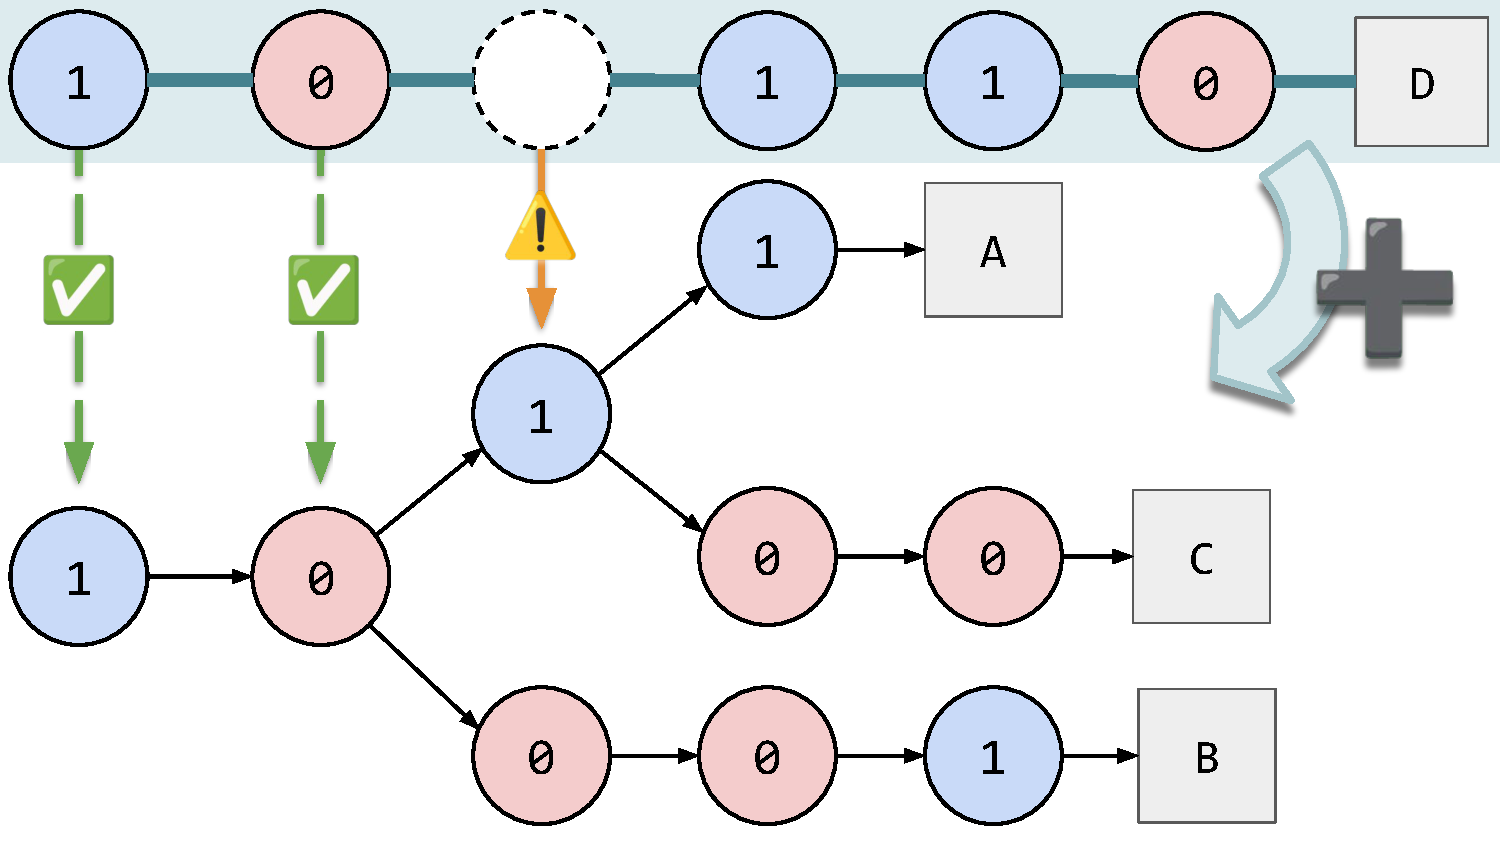
\includegraphics[width=\linewidth]{img/shortcut-algo-diagram-1}
  \subcaption{Preparing to add $D$}
  \label{fig:shortcut-algo-diagram-1}
\end{minipage}
\begin{minipage}{0.32\linewidth}
  \centering
  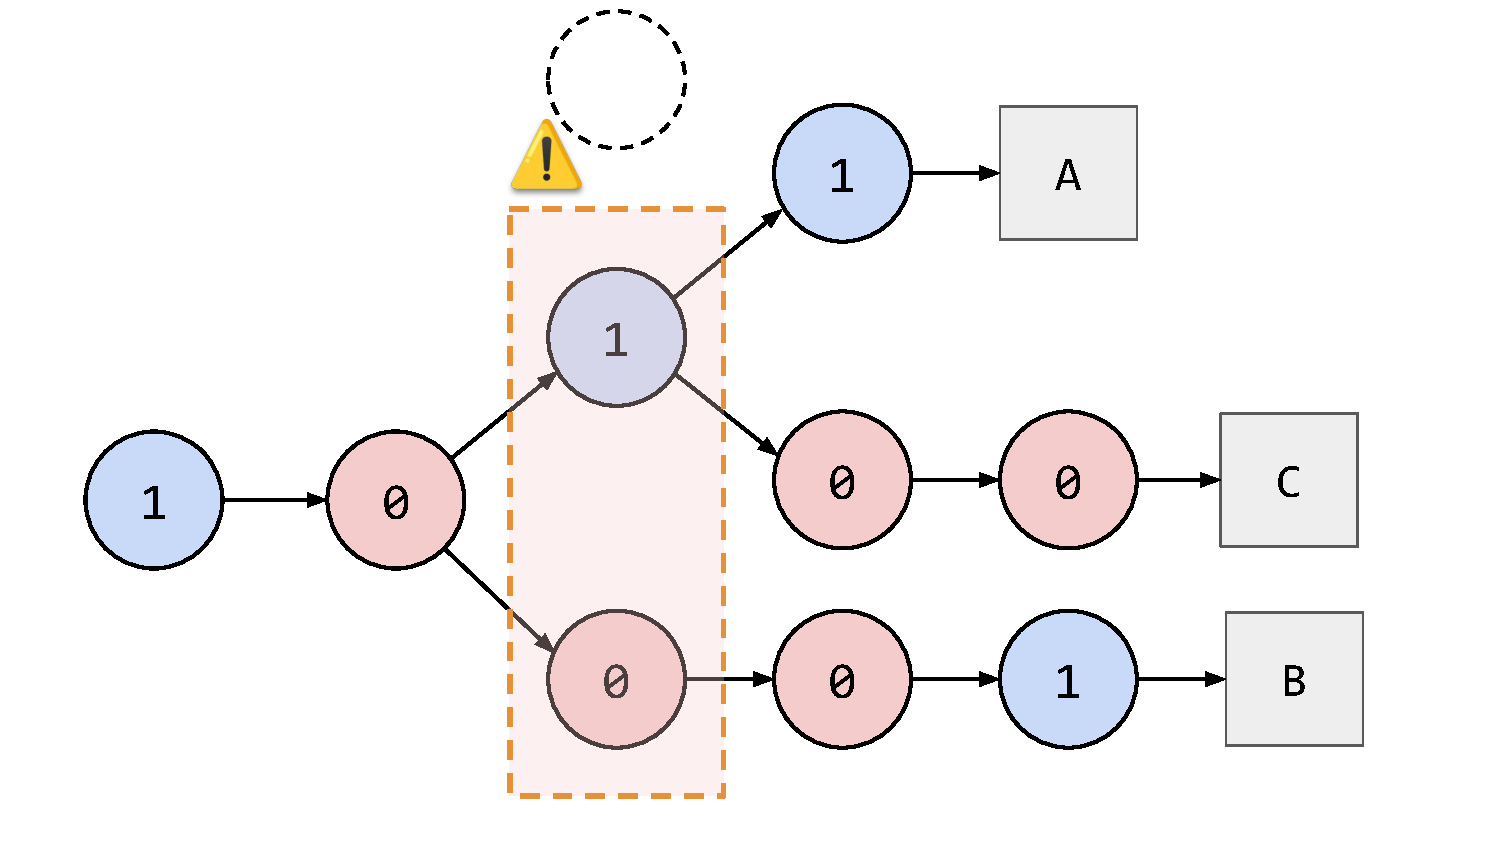
\includegraphics[width=\linewidth]{img/shortcut-algo-diagram-2}
  \subcaption{Encountering dropped marker}
  \label{fig:shortcut-algo-diagram-2}
\end{minipage}
\begin{minipage}{0.32\linewidth}
  \centering
  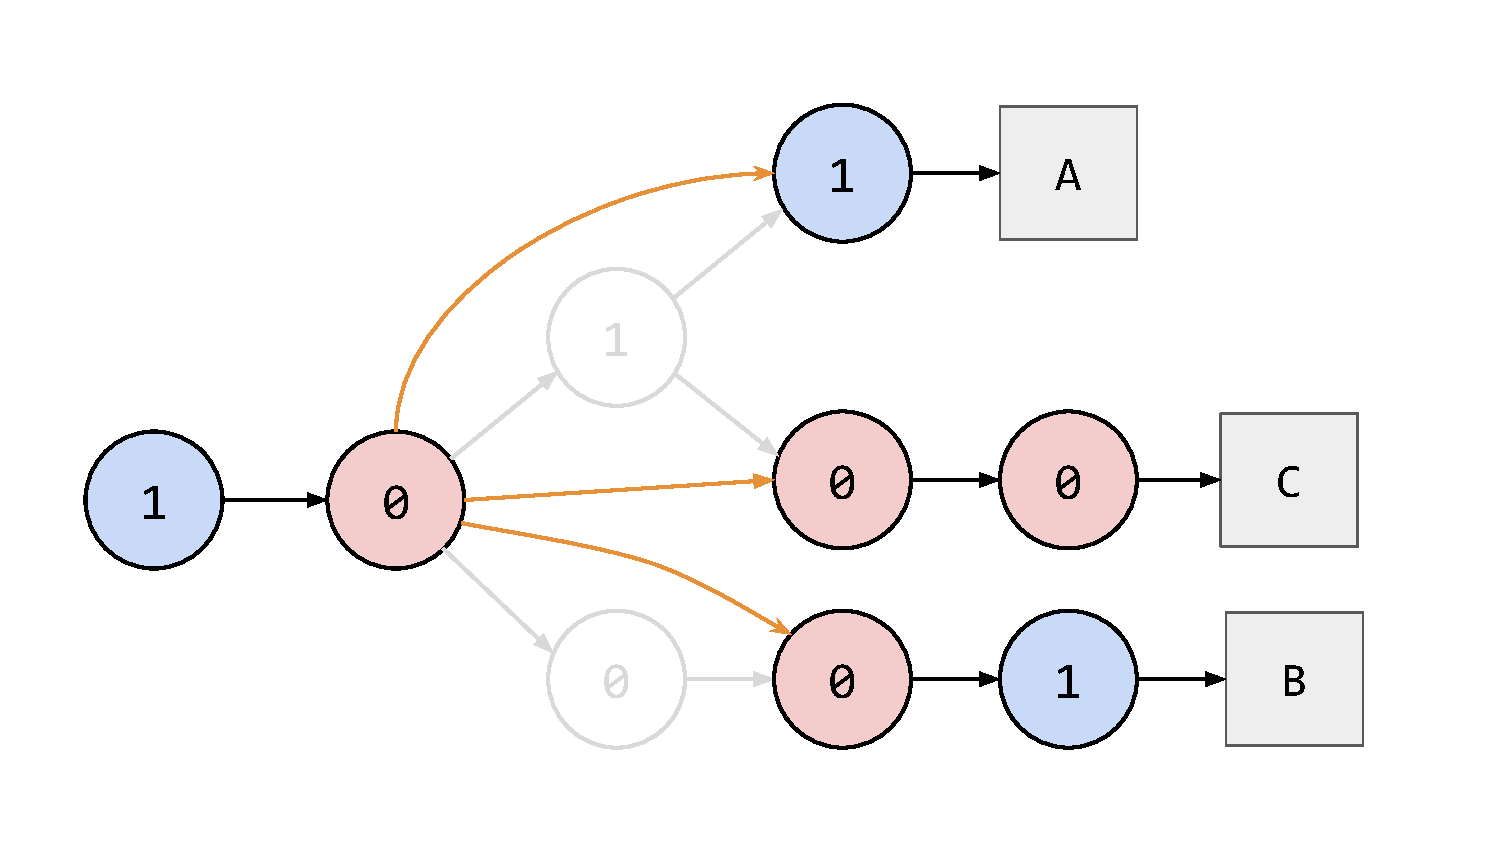
\includegraphics[width=\linewidth]{img/shortcut-algo-diagram-3}
  \subcaption{Building shortcuts}
  \label{fig:shortcut-algo-diagram-3}
\end{minipage}
\begin{minipage}{\linewidth}\par\end{minipage}
\begin{minipage}{0.32\linewidth}
  \centering
  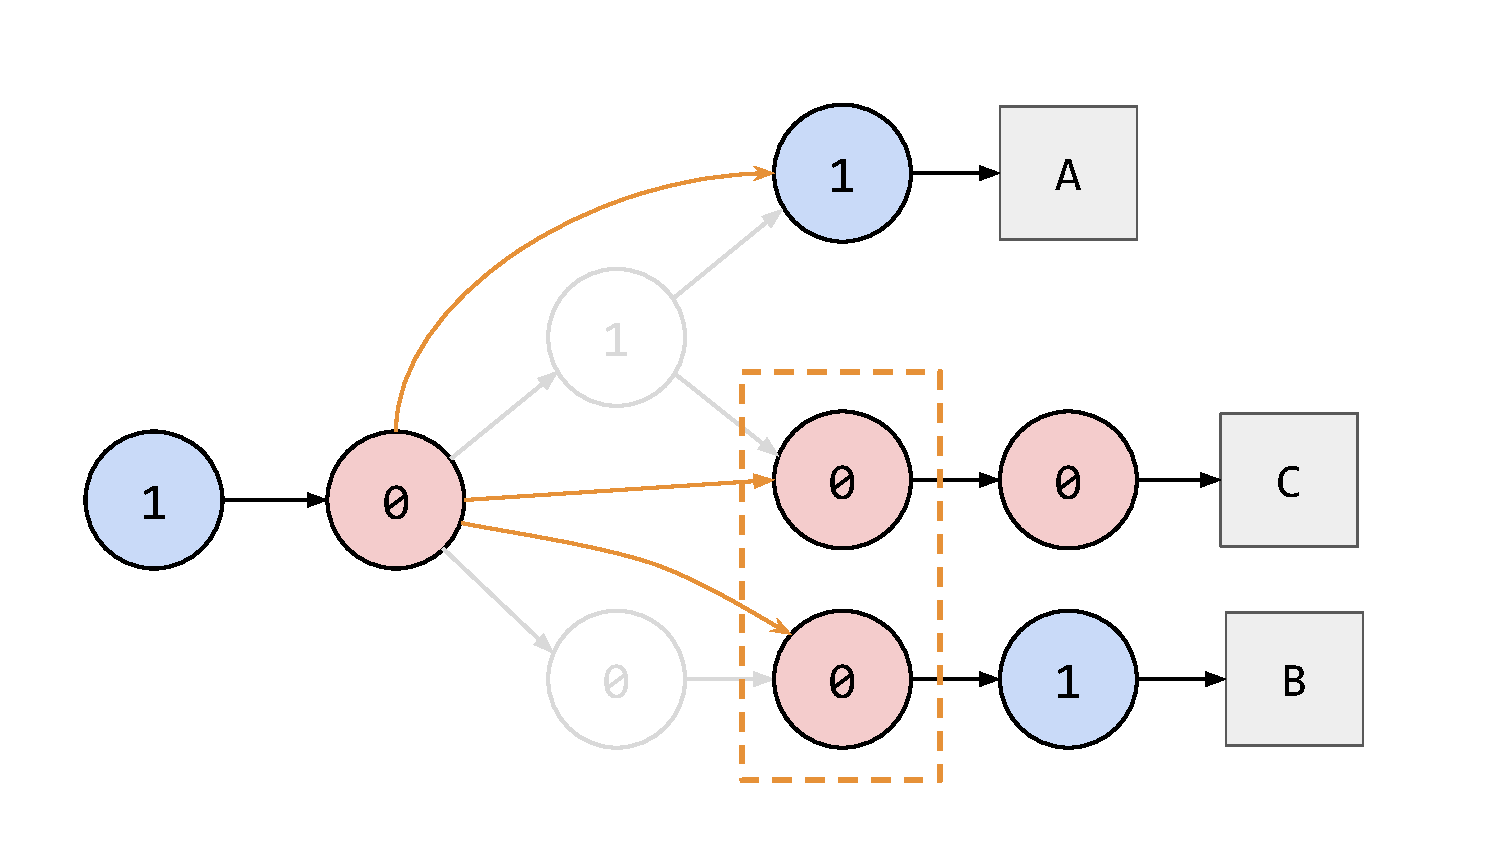
\includegraphics[width=\linewidth]{img/shortcut-algo-diagram-4}
  \subcaption{Indistinguishable nodes}
  \label{fig:shortcut-algo-diagram-4}
\end{minipage}
\begin{minipage}{0.32\linewidth}
  \centering
  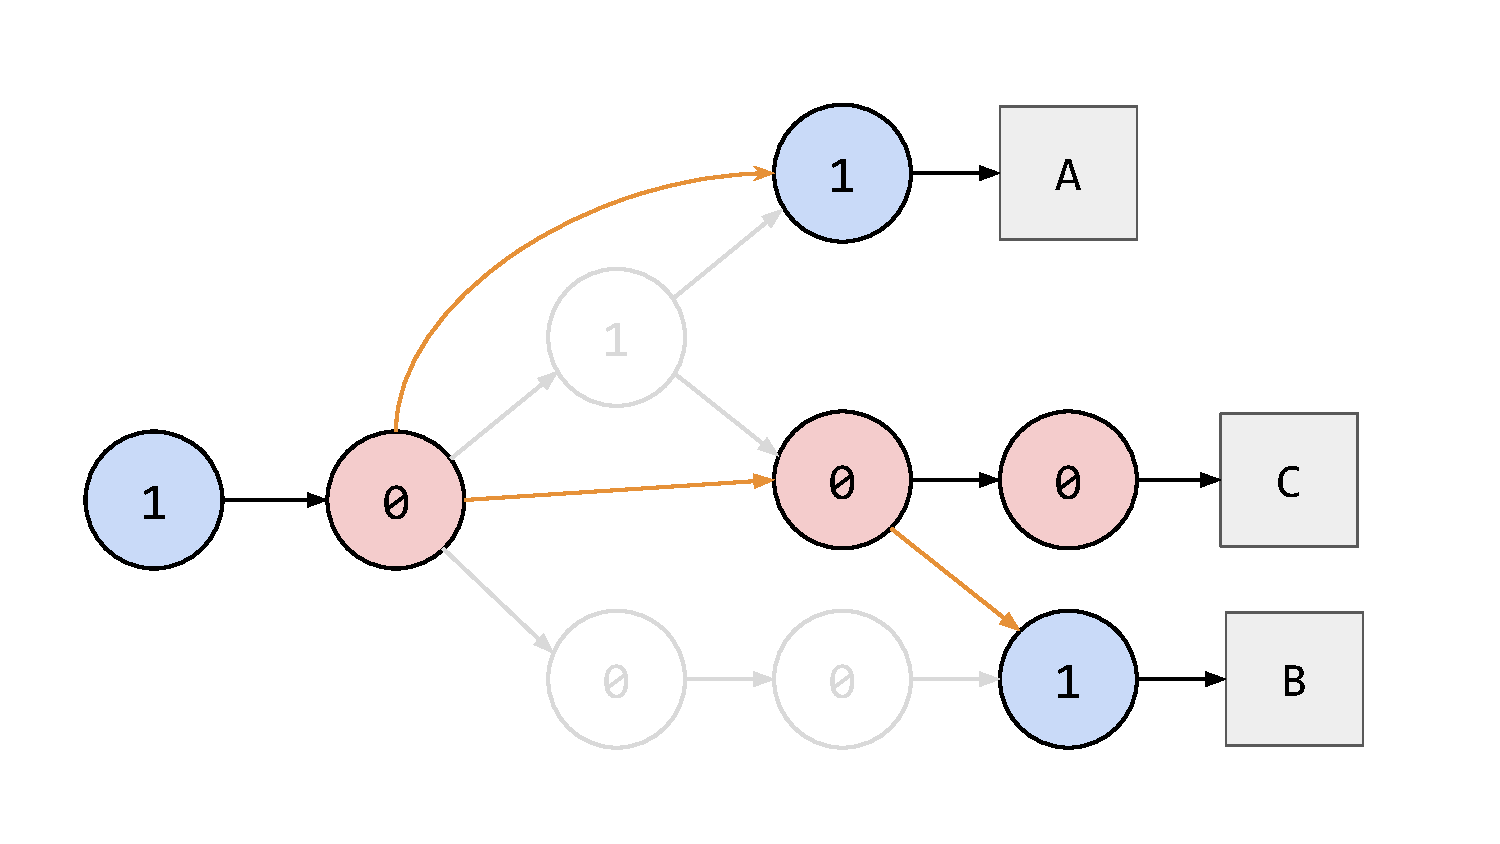
\includegraphics[width=\linewidth]{img/shortcut-algo-diagram-5}
  \subcaption{Collapsing redundant shortcuts}
  \label{fig:shortcut-algo-diagram-5}
\end{minipage}
\begin{minipage}{0.32\linewidth}
  \centering
  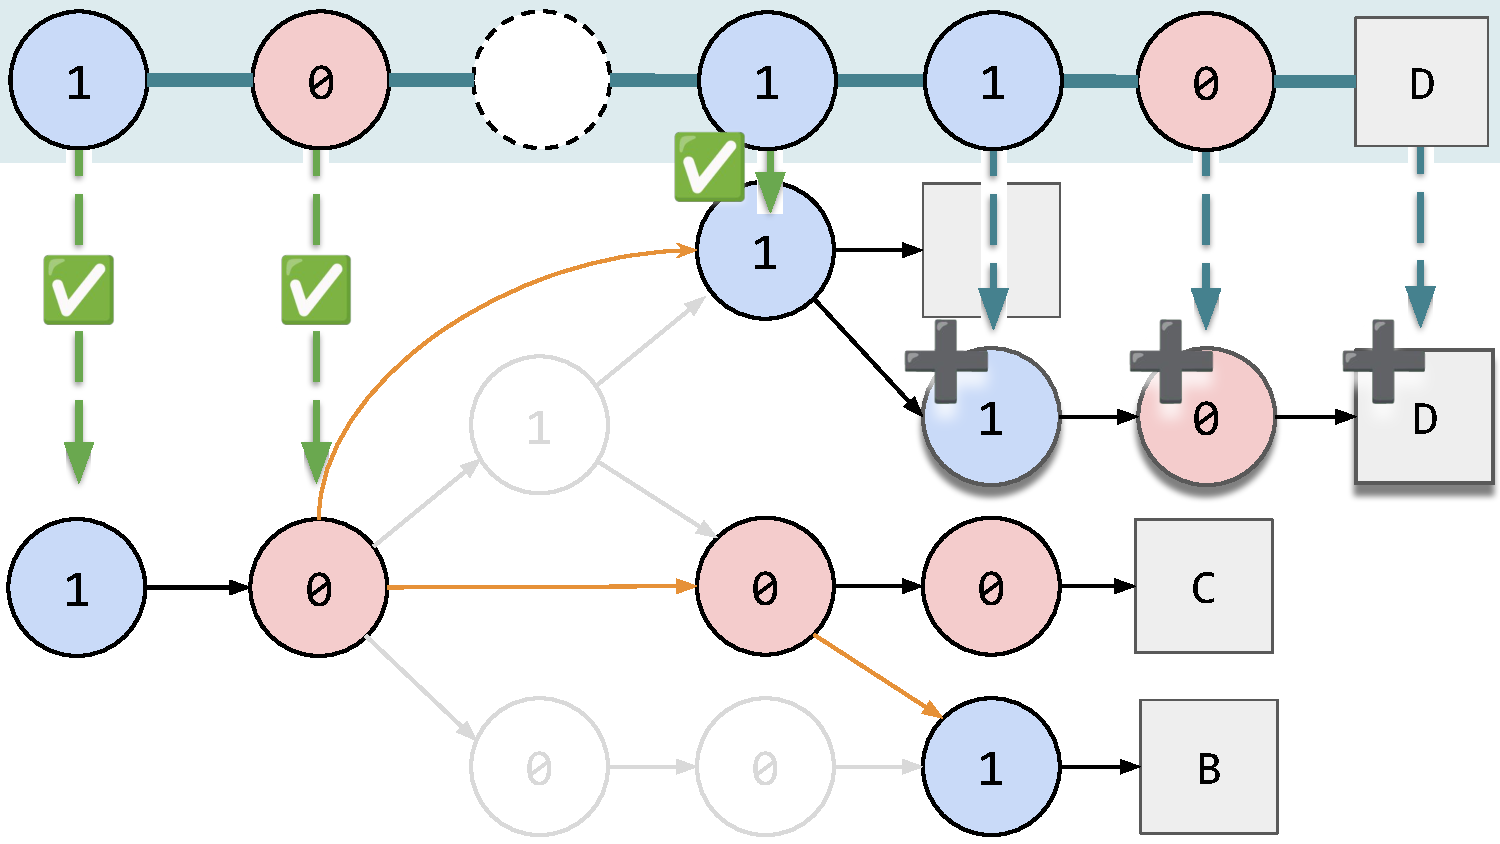
\includegraphics[width=\linewidth]{img/shortcut-algo-diagram-6}
  \subcaption{Organism $D$ added}
  \label{fig:shortcut-algo-diagram-6}
\end{minipage}
\end{minipage}
\begin{minipage}{0.24\linewidth}
\caption{%
\textbf{Trie-consolidation procedure for proposed shortcut algorithm.}
\small
A dropped hereditary marker is encountered while extending trie with genome $D$ (panel \ref{fig:shortcut-algo-diagram-2}).
All subsequent-added genomes will also have dropped markers at this position, so corresponding trie nodes may be bypassed by ``shortcut'' connections (panel \ref{fig:shortcut-algo-diagram-3}).
Note that bypassed trie structure is retained (``grayed-out'' nodes), so corresponding phylogenetic structure remains when reconstruction is finalized.
In a final step, shortcuts leading to identical nodes are further consolidated (panels \ref{fig:shortcut-algo-diagram-4} and \ref{fig:shortcut-algo-diagram-5}).
}
\label{fig:algo-diagram}
\end{minipage}
\vspace{-1.5em}
\end{figure*}


We propose a modification of Algorithm~\ref{alg:old} that replaces the $\textsc{MostLikelyChild}$ search in line 9 with a shortcut-building and consolidation step to deal with missing ranks.

Recall that once data from a specific rank is absent, it will not appear in any subsequent organisms.
Hence, trie nodes corresponding to that rank are no longer informative in placing subsequent data.
By building shortcuts bypassing such irrelevant nodes, we can speed up trie traversal for subsequent inserts.

In the shortcut-enabled approach, we detect missing information the same way as before: encountering some trie node $n'$ with a rank $r'$ that falls between the current organism $o$'s last-inserted rank $r_1$ and its currently-inserting rank $r_2$ (i.e., $r_1 < r' < r_2$).

Suppose we detect missing information while stepping from trie node $n$.
To proceed with shortcut construction, we will flesh out a full set $B$ of nearby no-longer-informative nodes.
We build $B$ by collecting all descendants of $n$ with rank $r''$ falling in the gap $r_1 < r'' < r_2$.
We then create shortcut edges that bypass nodes in $B$ --- connecting $n$ directly to the immediate descendants of $B$ with rank $\geq r_2$.

For illustration, see Figure~\ref{fig:algo-diagram}, where we detect a dropped rank (panel \ref{fig:shortcut-algo-diagram-2}) and create shortcut edges trie nodes with that dropped rank (panel \ref{fig:shortcut-algo-diagram-3}).
Edges to bypassed nodes $B$ are ignored in subsequent insert traversals, in favor of added shortcut edges.

One complicating factor may arise in shortcut construction: the introduction of ``indistinguishable nodes,'' where new sibling nodes happen to share the same rank and differentia value (like panel \ref{fig:shortcut-algo-diagram-4}).
This situation can be resolved by arbitrarily choosing one node to discard and transferring its children to the kept node using shortcut edges --- essentially `merging' the duplicates (panel \ref{fig:shortcut-algo-diagram-5}).

Algorithm~\ref{alg:consolidation} outlines steps for the described shortcut construction and consolidation procedure.
% Now, adding any organisms that are missing data from the removed level becomes trivial, as the algorithm can use the newly created shortcuts while skipping the missing information that was hidden by the consolidation step.
% We no longer need to look down branches from $n$ because the ``wildcard'' value has been eliminated --- each child of $n$ now has a rank greater than or equal to $r$.
% % So, there is no longer a concern of missing information when processing $n$ at rank $r$, and these shortcuts are then used to add any subsequent organisms if need be.
% If, at some point in the algorithm, $r$ itself becomes a rank of missing information, additional shortcuts are built according to the same procedure.

\begin{algorithm}[h]
  \begin{algorithmic}[1]
  \small{
    \Function{ConsolidateTree}{tree $T$, node $n$, rank $r$}
      \State $S \gets \{c \in \operatorname{descendants}(n) : \operatorname{rank}(c) \ge r \land  \operatorname{rank}(\operatorname{parent}(c)) < r\}$ 
      \For{$c$ in $S$} 
        \textsc{BuildShortcut}($T$, $n$, $c$)
      \EndFor
      \For{each subset of duplicate\footnotemark nodes $S' \subseteq S$}
        \State $c^* \gets$ an arbitrary element in $S'$ 
        \For{$c' \in S \setminus \{c^*\}$}
          \For{$c$ in $\operatorname{children}(c)$} 
            \State \textsc{BuildShortcut}($T$, $c^*$, $c$)
          \EndFor
          \State \textsc{RemoveShortcut}($T$, $n$, $c'$)
        \EndFor
      \EndFor 
    \EndFunction
    \Function{BuildShortcut}{tree $T$, node $n$, node $c$}
      \State $\operatorname{edges}(T) \gets \operatorname{edges}(T) \cup \{(n, c)\}$
      \State $\operatorname{edges}(T)[(n, c)]\text{.is\_shortcut} \gets \textsc{True}$
    \EndFunction
    \Function{RemoveShortcut}{tree $T$, node $n$, node $c$}
        \State $\operatorname{edges}(T) \gets \operatorname{edges}(T) \setminus \{(n, c)\}$
    \EndFunction
  }
  \end{algorithmic}
  \caption{\textbf{The consolidation step of the shortcut table algorithm.} \small Builds shortcuts for a given node $n$ and collapses duplicate children caused by those shortcuts. Note that \vspace{-1.5em}}
  \label{alg:consolidation}
\end{algorithm}
\footnotetext{nodes $x$ and $y$ are duplicates iff $\operatorname{rank}(x) = \operatorname{rank}(y)$ and $\operatorname{differentia}(x) = \operatorname{differentia}(y)$}

After insertion of the final organism into our trie, all that remains is to export a final phylogeny output.
At this stage, we ignore shortcut edges.
Crucially, while shortcut edges are useful for efficient traversal during insertions, they do not represent meaningful lineage relationships.
Instead, we use original trie edges as the basis for phylogeny output --- thereby preserving the full detail and granularity of the naive approach.
It is therefore necessary to retain records of the original trie structure, represented by light gray nodes and edges in Figure~\ref{fig:algo-diagram}.
Details about algorithm implementation and more detailed discussion of naive equivalency are provided in supplemental material \citep{supplemental}.
